%%%%%%%%%%%%%%%%%%%%%%%%%%%%%%%%%%%%%%%%%%%%%%%%%%%%%%%%%%%
%%%%%%%%%%%%%%%%% Theoretical calculations %%%%%%%%%%%%%%%%
%%%%%%%%%%%%%%%%%%%%%%%%%%%%%%%%%%%%%%%%%%%%%%%%%%%%%%%%%%%



\section{Study 1 - Modelling Signals}


%%%%%%%%%%%%%%%%% Theoretical calculations %%%%%%%%%%%%%%%%


\subsection{Theoretical calculations}


%%%%%%%%%%%%%%%%% First-order low-pass filter %%%%%%%%%%%%%


\subsubsection{First-order low-pass filter}

\begin{figure}[h]
\centering
\includegraphics[width=0.6\textwidth]{bilder/Lab1/Lab1fig1.eps}
\caption{PSD and ACF of first-order low-pass filter.}
\label{fig:Lab1fig1}
\end{figure}


%%%%%%%%%%%%%%%%% Ideal low-pass filter %%%%%%%%%%%%%%%%%%%


\subsubsection{Ideal low-pass filter}

\begin{figure}[h]
\centering
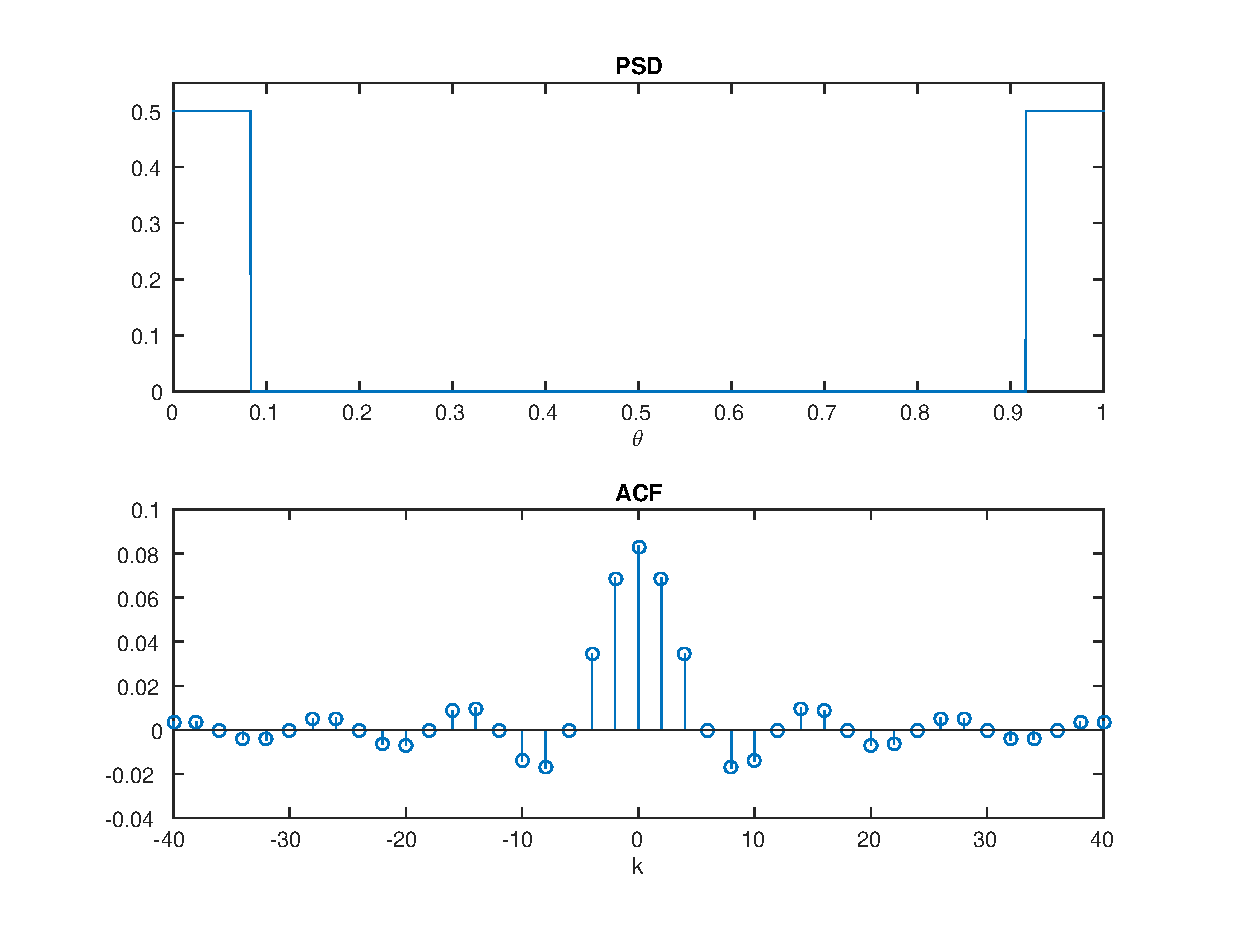
\includegraphics[width=0.8\textwidth]{bilder/Lab1/Lab1fig2.eps}
\caption{PSD and ACF of ideal low-pass filter.}
\label{fig:Lab1fig2}
\end{figure}


%%%%%%%%%%%%%%%%% Estimations %%%%%%%%%%%%%%%%%%%%%%%%%%%%%


\subsection{Estimations}


%%%%%%%%%%%%%%%%% Bartletts %%%%%%%%%%%%%%%%%%%%%%%%%%%%%%%


\subsubsection{Bartletts}

\begin{figure}[h]
\centering
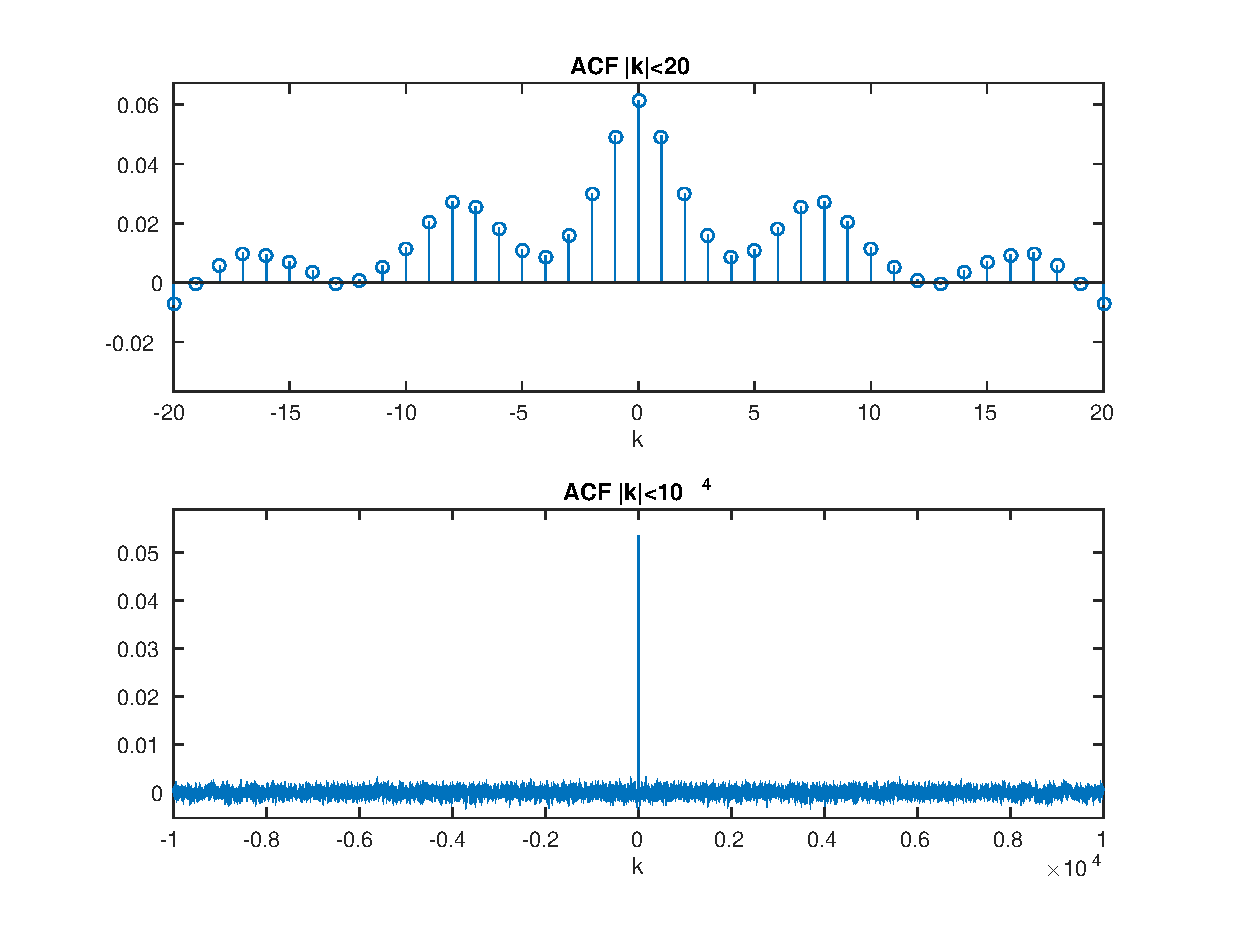
\includegraphics[width=0.8\textwidth]{bilder/Lab1/Lab1fig3.eps}
\caption{First-order low-pass ACF estimation.}
\label{fig:Lab1fig3}
\end{figure}

\begin{figure}[h]
\centering
\includegraphics[width=0.8\textwidth]{bilder/Lab1/Lab1fig4.eps}
\caption{High-order low-pass ACF estimate.}
\label{fig:Lab1fig4}
\end{figure}

\begin{figure}[h]
\centering
\includegraphics[width=0.8\textwidth]{bilder/Lab1/Lab1fig5.eps}
\caption{First-order low-pass PSD estimate.}
\label{fig:Lab1fig5}
\end{figure}

\begin{figure}[h]
\centering
\includegraphics[width=0.8\textwidth]{bilder/Lab1/Lab1fig6.eps}
\caption{High-order low-pass PSD estimate.}
\label{fig:Lab1fig6}
\end{figure}


%%%%%%%%%%%%%%%%% Improved estimations %%%%%%%%%%%%%%%%%%%%

\subsection{Improved estimations}


%%%%%%%%%%%%%%%%% Bartletts %%%%%%%%%%%%%%%%%%%%%%%%%%%%%%%

\subsubsection{Avering periodograms}

\begin{figure}[h]
\centering
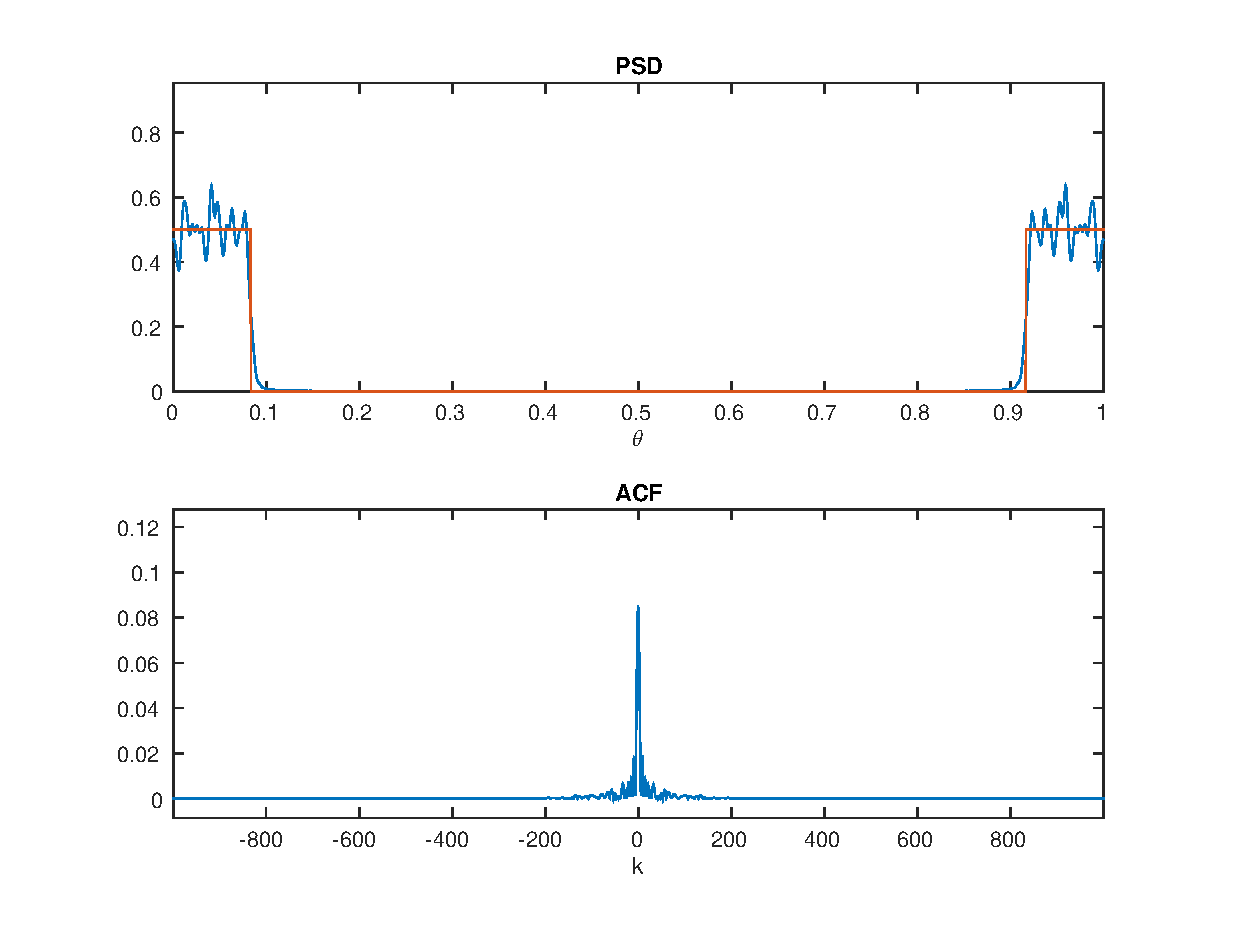
\includegraphics[width=0.8\textwidth]{bilder/Lab1/Lab1fig8.eps}
\caption{Low-order low-pass PSD and ACF improved estimates.}
\label{fig:Lab1fig8}
\end{figure}

\begin{figure}[h]
\centering
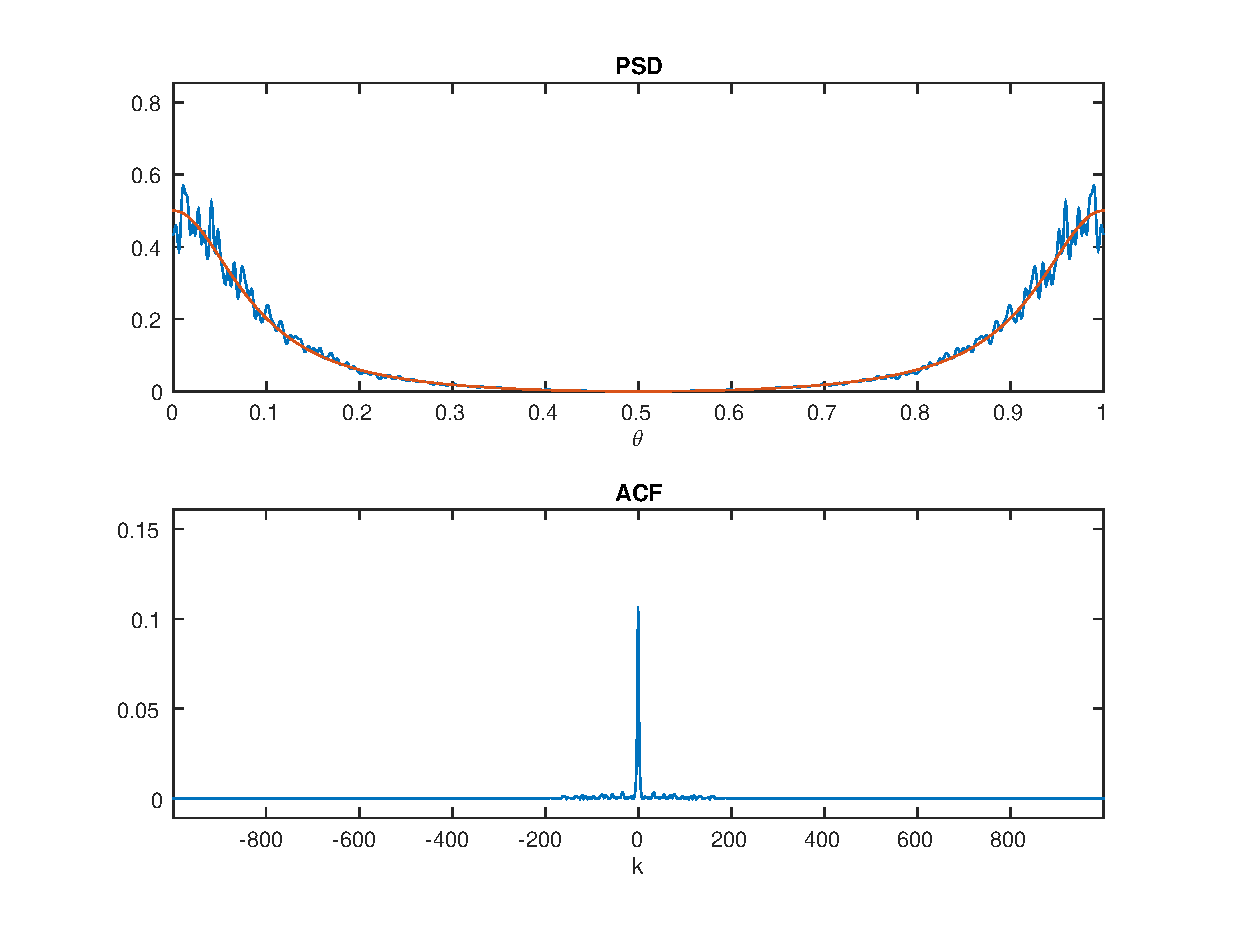
\includegraphics[width=0.8\textwidth]{bilder/Lab1/Lab1fig7.eps}
\caption{High-order low-pass PSD and ACF improved estimates.}
\label{fig:Lab1fig7}
\end{figure}


%%%%%%%%%%%%%%%%% Bartletts %%%%%%%%%%%%%%%%%%%%%%%%%%%%%%%

\subsubsection{Smoothing}

\begin{figure}[h]
\centering
\includegraphics[width=0.8\textwidth]{bilder/Lab1/Lab1fig11.eps}
\caption{Some diffrent windows used in smoothing.}
\label{fig:Lab1fig11}
\end{figure}

\begin{figure}[h]
\centering
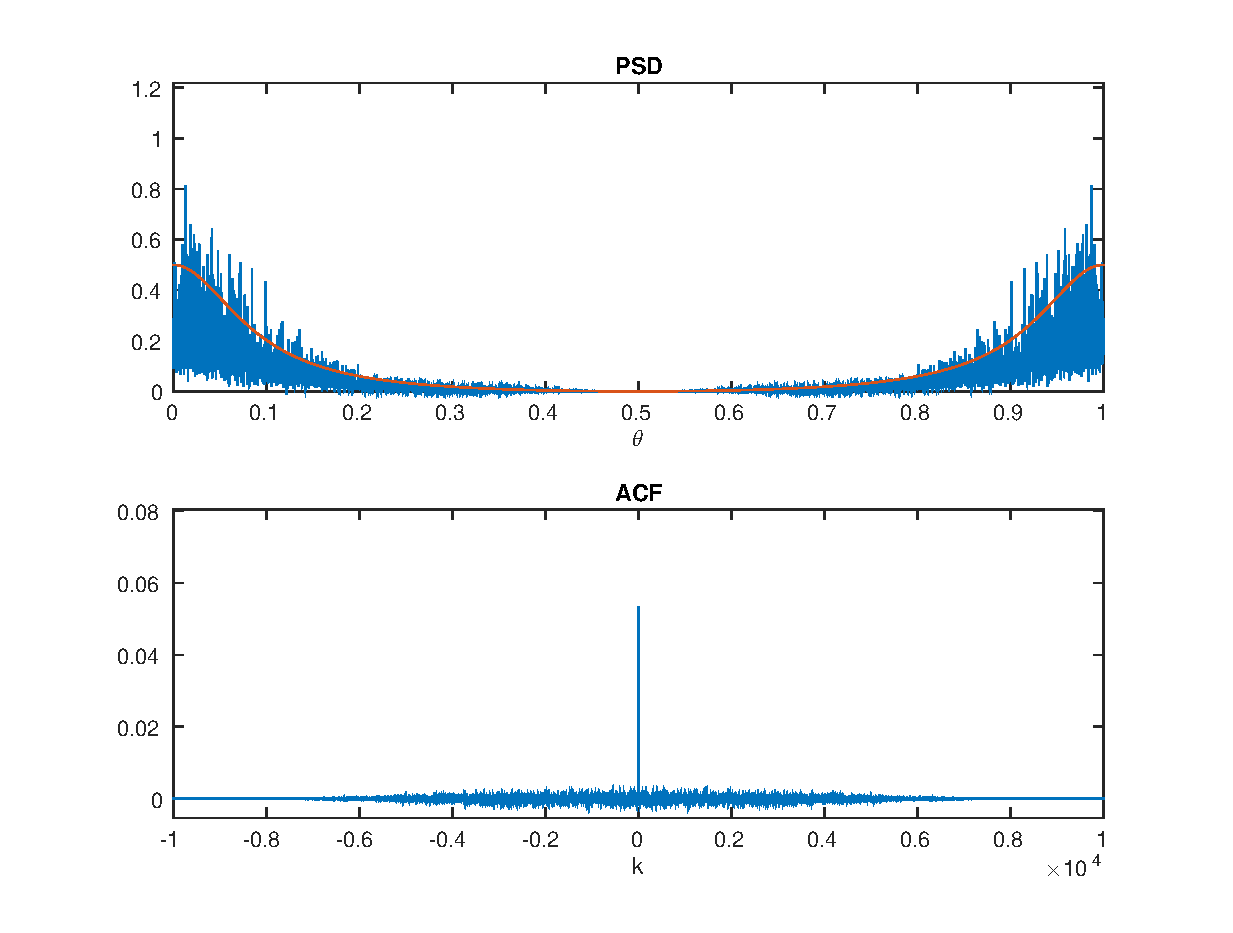
\includegraphics[width=0.8\textwidth]{bilder/Lab1/Lab1fig9.eps}
\caption{Low-order low-pass ACF and PSD improved estimate.}
\label{fig:Lab1fig9}
\end{figure}

\begin{figure}[h]
\centering
\includegraphics[width=0.8\textwidth]{bilder/Lab1/Lab1fig10.eps}
\caption{High-order low-pass ACF and PSD improved estimate.}
\label{fig:Lab1fig10}
\end{figure}


%%%%%%%%%%%%%%%%% Discussion %%%%%%%%%%%%%%%%%%%%%%%%%%%%%%

\subsection{Discussion}
